\chapter{Metastability and phononic CDW quench in TaTe2}

Strongly correlated condensed matter systems are materials with a very high complexity, making it difficult to predict and understand their properties.
To reduce this complexity Novoselov, Geim and co-workers proposed Graphene as a model system for more complex materials \cite{novoselov_electric_2004, novoselov_two-dimensional_2005, geim_rise_2007}.
Since then, researchers were extremely successful in finding new physical properties of Graphene itself while also extending and applying the knowledge to other materials.
Apart from the simplicity of these 2D materials, the idea of engineering properties by stacking multiple layers with different stacking orders or at twist angles offered the possibility of a vast playground for discovering and engineering new properties.
This resulted in the explosion of the field with the discovery of many new phenomena, from the observation of quatum Hall effect \cite{zhang_experimental_2005} to superconductivty in magic angle twisted bilayer graphene \cite{cao_unconventional_2018}.
Ultimately these developments lead the emergence other 2D material platforms.
One of these platforms of 2D materials are transition metal dichalcogenides (TMDs) \cite{butler_progress_2013, chowdhury_progress_2020, liu_van_2016}.

These layered TMDs exhibit various phenomena xyz


One constituent of these TMDs is \ce{TaTe2} which, compared to its \ce{TaX2} based sister compounds \ce{TaS2} and \ce{TaSe2} and the isostructural polytypes of \ce{MTe2} like \ce{NbTe2} or \ce{VTe2}, it has so far received less attention from the community, but some reports characterizing the compound have come up in recent years, as well as the first ultrafast out-of-equilibrium studies.

Here talk more about the MTe and TaX properties (see RRR intro)

\ce{TaTe2} can be characterized as a semimetal at room temperature (RT), which forms ribbon like structures in a distorted (3 x 1) 1T'-phase.
The compound appears to have strong molecular properties, with \ce{Ta} atoms forming in trimers or fluctuating dimers, with each \ce{Ta}-atoms being surrounded by 8 \ce{Te}-atoms.
At \SI{170}{\kelvin} the material undergoes a structural phase transitions, where two \ce{Ta}-atoms further distort the structure, breaking dimers and instead form "butterfly" shaped heptameres in a (3 x 3) 1T"-phase \cite{feng_charge_2016, katayama_observation_2023}.
This structural phase transition is accompanied by the formation of charge density wave (CDW), which has been observed both by gap formation in ARPES \cite{lin_evidence_2022, mitsuishi_unveiling_2024} and the formation of a periodic lattice distortion (PLD) in STM and diffraction \cite{feng_charge_2016, siddiqui_ultrafast_2021, domrose_femtosecond_2024}.
The exact mechanism of how this phase transition occurs and what the interplay with the CDW is have still not been understood.

\begin{figure}
	\centering
	\begin{subfigure}[b]{0.3\textwidth}
		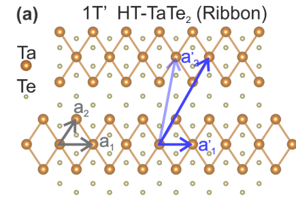
\includegraphics[width=\textwidth]{tate2/ht_structure.png}
	\end{subfigure}
	\hfill
	\begin{subfigure}[b]{0.3\textwidth}
		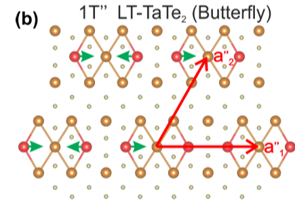
\includegraphics[width=\textwidth]{tate2/lt_structure.png}
	\end{subfigure}
	\hfill
	\begin{subfigure}[b]{0.3\textwidth}
		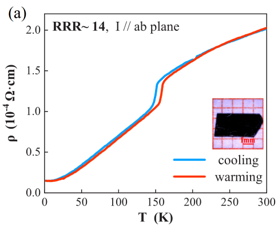
\includegraphics[width=\textwidth]{tate2/resistivity.png}
	\end{subfigure}
	\caption{(a) 1T' RT phase of \ce{TaTe2} forming ribbons. (b) 1T" LT phase of \ce{TaTe2}, \ce{Ta} atoms move together forming heptameres. (c) Resistivity of \ce{TaTe2} as a function of temperature with an overall reduction in resistivity while cooling. A phase transition occurs at \SI{170}{\kelvin}, which is accompanied by a further steplike reduction in resistivity.}
	\label{fig:tate_structure}
\end{figure}


The reason for the lack of understanding stems from the electronic reaction to the phase transition, especially in comparison to the \ce{TaX2} sister compounds.
Typically, entering a CDW phase by cooling the sample down from RT leads to an increase in resistivity due to the reduced density of states (DOS) in proximity to the Fermi level $E_F$.
Similarly a drop of the magnetic susceptibility would be expected while cooling $T_s$.
Instead \ce{TaTe2} shows a drop in resistivity and an increase in magnetic susceptibility, despite the observation of small gaps in the band structure \cite{sorgel_new_2006,hu_optical_2022,lin_evidence_2022}.
For this reason the compound has been branded a "strange" CDW material.

In this chapter of the thesis I give further insight into the driving mechanism of the CDW and the formation of the structural phase transition with the help of ultrafast pump-probe ARPES, and comparing our data to the recent ARPES and ultrafast publications on \ce{TaTe2}.
I will first introduce the band structure of \ce{TaTe2} and the Fermi surface topology, comparing the RT and LT phase, including the formation of CDW minigaps (first observed by \cite{lin_evidence_2022}).
After this I will give a description of the charge dynamics on a few picosecond timescale, including the delayed response of the CDW.
And then focus on the strong, band specific oscillations observed in the time domain and analyzing the different oscialltion modes with the help of Fourier analysis.
Last, I present a metastable electronic state persisting for $>\SI{200}{\pico\second}$ and discuss it's relevancy for the phase structural phase transition at equilibrium.

\section{Bandstructure and Fermiology}

The electronic structure of \ce{TaTe2} is characterized by the strong molecular bonding properties of the Ta-Ta dimers, with a strong orbital character.
Studying the band structure with ARPES reveals a complex set of bands at RT.
The valence states, which are governing the electronic properties of the compound consist of a mix of Ta 5d and Te 5p orbitals. \cite{mitsuishi_unveiling_2024}

The Fermi surface of \ce{TaTe2} shows a much stronger quasi-1D character when compared to other 2D materials, even the isostructural \ce{TaSe2} and \ce{TaS2}.
This character can be observed by 2-fold symmetric wavy contours around \SI{0.5}{\angstrom^{-1}}, which are located along the $\Gamma$-M$_1$ direction and forms an outer Fermi surface.
Within these contours, an inner second Fermi surface forming multiple pockets can be located (see Fig. \ref{fig:TaTe_FS}).

\begin{figure}[h!]
	\centering
	\begin{subfigure}[b]{0.5\textwidth}
		\includegraphics[width=\textwidth]{tate2/TaTe2_BZ_sketch_full.pdf}
		\caption{}
	\end{subfigure}
	\hfill
	\\
	\begin{subfigure}[b]{0.49\textwidth}
		\includegraphics[width=\textwidth]{tate2/TaTe2_FS_RT.pdf}
		\caption{}
	\end{subfigure}
	\hfill
	\begin{subfigure}[b]{0.49\textwidth}
		\includegraphics[width=\textwidth]{tate2/TaTe2_FS_LT.pdf}
		\caption{}
	\end{subfigure}
	\caption{(a) The measured Fermi surface of the LT phase is overlapped with the 1. BZ of the virtual monoclinic (1 x 1) 1T phase (black), extended BZs of the distorted HT (3 x 1) 1T' phase (orange) and extended BZs of the further distorted LT (3 x 3) 1 T'' phase (red). (b) RT Fermi surface overlapped with the HT and LT Brillouin zones. The relevant high symmetry points are marked. (c) Same Fermi surface as (b) but measured in the LT phase at \SI{77}{\kelvin}.}
	\label{fig:TaTe_FS}
\end{figure}

Comparing the RT and LT Fermi surface, only small changes can be observed.
The overall topology, consisting of the wavy outer contours and an inner FS sheet with multiple pockets is conserved.
A main difference lies in the slightly changed size of the pockets in the inner sheet, as some more pronounced features in the 2nd BZ of the LT FS.
The difference in size of the pockets stems from a slightly shifted chemical potential, when cooling through the phase transition, which has also been observed by N. Mitsuishi et. al. \cite{mitsuishi_unveiling_2024}.

Instead of the small changes in the Fermi surface topology, the effects of the phase transition become apparent when investigating the EDCs.
Here, we compare a series of EDCs taken parallel to the K$_1$-$\Gamma$-K$_1$ direction from the $\Gamma$-point to the edge of the 2nd BZ, for both room and low temperature.

\begin{figure}[t!]
	\centering
	\includegraphics[width=0.9\textwidth]{tate2/TaTe2_RT_cuts.pdf}
	\caption{Series of cuts parallel to K$_1$-$\Gamma$-K$_1$, from $\Gamma$ to the BZ border. The location of the cuts in respect to the BZ is indicated in the FS of Fig. \ref{fig:TaTe_FS}. All cuts have been taken at RT, using the Helium $\alpha1$ line of a Helium lamp.}
	\label{fig:TaTe_RT_cuts}
\end{figure}

The RT EDCs show a manifold of bands, with multiple bands crossing the Fermi level in each cut.
These Fermi crossings clearly show the two different Fermi sheets, with the crossing at the edge of the cut determining the wavy contours of the outer quasi-1D Fermi surface sheet, and the crossing close to the center of the band structure forming the 2nd, inner Fermi sheet.
Cooling the compound through the phase transition results in a complex reordering of the bands.
The broader bands from the RT phase seem to split in multiple individual ones, with additional backfolded bands appearing.
Looking at the FS crossing of the inner sheet, the aforementioned size difference it the Fermi pockets becomes clearer.
Comparing the cuts of the RT phase to the equivalent LT cuts, it is possible to identify a small shift in the chemical potential $\mu$, which has also been reported by \cite{mitsuishi_unveiling_2024}.
Another difference between the two phases seems to lie in the flattening of the band dispersion close to $E_F$ at energies above \SI{-0.6}{\electronvolt}.

\begin{figure}[h]
	\centering
	\includegraphics[width=0.9\textwidth]{tate2/TaTe2_LT_cuts.pdf}
	\caption{Series of cuts parallel to K$_1$-$\Gamma$-K$_1$, from $\Gamma$ to the BZ border. The cuts are the equivalent band maps to the RT one in Fig. \ref{fig:TaTe_RT_cuts}. All cuts have been taken at LT $\simeq$\SI{77}{\kelvin}, using the Helium $\alpha1$ line of a Helium lamp.}
	\label{fig:TaTe_LT_cuts}
\end{figure}

This flattening of the bands might stem from the established charge order due to the CDW phase, typically resulting in the opening of gaps and backfolded bands from the PLD.
To further address the CDW and the gap formation we have to revisit the quasi-1D character of the FS.
A nesting of the FS occurs when different parts of the Fermi surface can be connected by a reciprocal lattice vector which can translate the different parts on top of each other.
This Fermi surface nesting (FSN) leads then to charge instabilities close to the FS and can play a dominant role in the formation of CDWs.
The wavy contours of the outer FS sheet (see Fig. \ref{fig:TaTe_FS}) fulfill the Fermi surface nesting (FSN) conditions.
Determining the distance between two points that are connected by this vector results in a length of approximately \SI{0.92}{\angstrom^{-1}}, which is comparable to the \SI{0.85}{\angstrom^{-1}} found by Y. Lin et al. \cite{lin_evidence_2022}.
A possible second FSN vector can be found for the inner FS sheet.
These bands show a stronger 1D character and the vector has a length of \SI{0.24}{\angstrom^{-1}}.
Both of these FSN vector lengths do not correspond to the periodicity of the PLD, which was found to be $\simeq\SI{0.67}{\angstrom^{-1}}$.
The discrepancy between these vector lengths means that the FSN is not the sole driving force of the phase transition, underlining the complexity of the situation in \ce{TaTe2}.

As a result of the CDW formation minigaps can be observed across the Brillouin zone, most prominently close to the $\Gamma$-point \cite{lin_evidence_2022}.
Figure \ref{fig:TaTe_minigaps} shows a cut close to $\Gamma$, with a dashed box around the area in which the minigap formation occurs.
A zoom of this region better showcases these small gaps at the edge of the band map at around \SI{0.4}{\angstrom^{-1}}.
This band also connects to the wavy contours, which fulfill the FSN condition, further underlining the relevance for the CDW.

\begin{figure}[h!]
	\centering
	\includegraphics[width=0.7\textwidth]{tate2/TaTe2_CDW_minigaps.pdf}
	\caption{Left: Band map parallel to the K$_1$-$\Gamma$-K$_1$ direction close to the $\Gamma$-point. The dashed rectangle marks the region of which a zoom is provided. Right: Zoom of dashed rectangle region. The band map shows a faint signature of the observed minigaps \cite{lin_evidence_2022}.}
	\label{fig:TaTe_minigaps}
\end{figure}

\section{Ultrafast charge dynamics and CDW quench}

Investigating the evolution of the electronic band structure after pump excitation provides insight into the relaxation dynamics, not only of an isolated electronic states, but also the influence of the system.
Performing pump-probe experiments at RT and LN temperature allows us to reveal differences between the two different structural phases.
The excitation is created by a \SI{1.55}{\electronvolt} pulse.
Here I will first analyze measurements that have been performed in the low temperature phase at \SI{77}{\kelvin} and then switch to RT data to point out the differences due to the phase transition.

The LT cuts, presented in this section, have been measured parallel to K$_1$-$\Gamma$-K$_1$ direction at three different points in the LT FBZ ($\Gamma$, M$_1$ and in proximity of $\Gamma$ See Fig. ref).
Focusing on the cut close to $\Gamma$ it is possible to make out a complex band dynamics, depending on the region in the band structure.
Figure \ref{fig:TaTe_bandmap_dyn_betw} shows this band map \SI{50}{\femto\second} after excitation.
Additionally, difference maps for three different time steps (\SIlist{50; 500; 4000}{\femto\second}) are plotted to better display the pump induced changes.

At \SI{50}{\femto\second} a fast depopulation of occupied bands can be observed, with the difference band contours following the band structure at equilibrium.
Similarly a fast population of the unoccupied states occurs.
After a decay of the excitation sets in as expected, but at \SI{500}{\femto\second} a sudden increase in spectral weight occurs in the occupied states.
This atypical behavior can be explained by a quench of the charge order, and will be discussed in greater detail when analyzing the specific delay traces.
At a time delay of \SI{4}{\pico\second} most of the population in the excited states has decayed, but a rest population is still observed.
Additionally the band structure is significantly altered compared to the equilibrium state.

\begin{figure}[t!]
	\centering
	\includegraphics[width=\textwidth]{tate2/bandmap_dyn_markers_betw.pdf}
	\caption{Left: Band map close to $\Gamma$ oriented along K$_1$-$\Gamma$-K$_1$ direction at a time delay of \SI{50}{\femto\second} after pump excitation. The other plots show difference maps at different time delays (\SIlist{50;500;4000}{\femto\second}). Rectangles show the regions for which dedicated delay traces are displayed in \ref{fig:TaTe_dyn_betw}. The difference map show characteristic features for each time steps. At \SI{50}{\femto\second} fast de-/population due to the pump excitation occurs. After \SI{500}{\femto\second} a population of a region below $E_F$ appears, corresponding to the closure of the CDW gap. After \SI{4}{\pico\second} the difference map shows regions where a change of the band structure and population above $E_F$ persists. Measurement was done at \SI{77}{\kelvin}.}
	\label{fig:TaTe_bandmap_dyn_betw}
\end{figure}

Some exemplary traces have been selected for a more detailed insight into the relaxation dynamics.
These traces are marked with squared in the band maps, black squares for the unoccupied band structure, white for the occupied region and green for the region with a significant spectral weight after \SI{4}{\pico\second}.
Traces for the unoccupied region (black squares, see Fig. \ref{fig:TaTe_dyn_betw} (a)-(c)) shows a sharp population within the duration of the pump pulse.
The ultrafast population is followed by a fast decay which becomes increasingly longer when approaching $E_F$, in accordance with the scattering rate $\tau \propto \sqrt{E-E_F}$.
In each trace, the population has decayed within \SI{4}{\pico\second}.
Similarly the depopulation of the occupied state in Fig. \ref{fig:TaTe_dyn_betw} (d) is created within the pump pulse duration and recovers on the same time scale.

Unexpected dynamics occur when looking at the region that shows a increase in population below $E_F$.
Typically a pump light pulse excites the system which transfers energy to electrons and driving a transition to a higher unoccupied state, therefore reducing the occupancy below $E_F$.
Instead \ce{TaTe2} shows small gaps resulting from the CDW, which leads in the LT phase to a loss of density of states (DOS), when compared to the RT phase.
If this charge order is broken, the gap closes and in a simple case, excluding other band modifications, the DOS of the RT phase is re-established.
This behavior is observed in Fig. \ref{fig:TaTe_dyn_betw} (e), which coincides with the region of CDW gaps reported by \cite{lin_evidence_2022}.
Strikingly, the breaking of the CDW order does not occur at $t_0$.
Fitting a single exponential decay model retrieves a time zero of $t_0=\SI{388}{\femto\second}$, introducing a significant delay of approximately \SI{320}{\femto\second} when compared to the time zero of all other curves.

This delayed response becomes very apparent, when the delay trace is overlapped with the dynamics of the fast de- or population (see Fig. \ref{fig:TaTe_CDW_comp}).
In most studies on CDW hosting materials the respective is quenched instantaneously after pump excitation, underlining the electronic behavior of the charge order.
Here, the clear delayed response rules out a solely electronic character and instead established the structural component as the dominant contribution for the CDW order in \ce{TaTe2}.
In other words, instead of the electromagnetic field of the pump pulse directly disrupting the charge order, the more likely scenario is an impulsive response of the lattice to the intense light illumination, resulting in an excitation of phonon modes on ultrafast time scales, which couple to the charge order via the strong electron-phonon coupling of the system.

\begin{figure}[t]
	\centering
	\begin{subfigure}[b]{0.33\textwidth}
		\includegraphics[width=\textwidth]{tate2/Unocc_dyn_1_fit_betw.pdf}
		\caption{}
	\end{subfigure}
	\hfill
	\begin{subfigure}[b]{0.33\textwidth}
		\includegraphics[width=\textwidth]{tate2/Unocc_dyn_2_fit_betw.pdf}
		\caption{}
	\end{subfigure}
	\hfill
	\begin{subfigure}[b]{0.33\textwidth}
		\includegraphics[width=\textwidth]{tate2/Unocc_dyn_3_fit_betw.pdf}
		\caption{}
	\end{subfigure}
	\\
	\begin{subfigure}[b]{0.33\textwidth}
		\includegraphics[width=\textwidth]{tate2/Occ_dyn_fit_betw.pdf}
		\caption{}
	\end{subfigure}
	\hfill
	\begin{subfigure}[b]{0.33\textwidth}
		\includegraphics[width=\textwidth]{tate2/CDW_quench_fit_betw.pdf}
		\caption{}
	\end{subfigure}
	\hfill
	\begin{subfigure}[b]{0.33\textwidth}
		\includegraphics[width=\textwidth]{tate2/Meta_dyn_fit_betw.pdf}
		\caption{}
	\end{subfigure}
	\caption{Delay traces of the regions marked in Fig. \ref{fig:TaTe_bandmap_dyn_betw} with the corresponding fit function of a single exponential decay model and resulting time constants $t_0$ and $\tau$. (a)-(c) Dynamics of unoccupied regions (black markers in Fig. \ref{fig:TaTe_bandmap_dyn_betw}) show fast population within pump pulse, followed with increasing relaxation time closer to $E_F$. (d)-(e) Dynamics of unoccupied regions (white markers in Fig. \ref{fig:TaTe_bandmap_dyn_betw}). (d) Fast depopulation within pump excitation. (e) Delayed response compared to $t_0$ and increased spectral weight. (f) Dynamics of region slightly above $E_F$ (green marker in Fig. \ref{fig:TaTe_bandmap_dyn_betw}) shows a instantaneous population within pump pulse, and persisting occupation beyond \SI{4}{\pico\second}.}
	\label{fig:TaTe_dyn_betw}
\end{figure}

The unresponsiveness of the CDW to the direct light illumination shows as well when looking at a region at the edge of the CDW gap, also containing the part of the gapped band.
The corresponding dynamics, overlapped with the dynamics of the direct de-/population are shown in Fig. \ref{fig:TaTe_CDW_comp}.
In the trace an inital dip at $t_0$ can be seen, originating from the depopulation dynamics of the occupied band.
But after \SI{300}{\femto\second}, this depopulation is downed out by the closing of the CDW gap.
It is quite remarkable that in adjacent energy-momentum coordinates an instantaneous reaction to the occupied band dynamics is observed while the CDW only shows a delayed response, which speaks for the strong structural character of the established order.
A relaxation time of $\tau_{CDW}=\SI{500}{\femto\second}$ can be extracted by fitting a single exponential decay model, corresponding to the time duration to reestablish the charge order.

\begin{figure}[t!]
	\centering
	\begin{subfigure}[b]{0.33\textwidth}
		\includegraphics[width=\textwidth]{tate2/CDW_quench_multitrace_betw.pdf}
		\caption{}
	\end{subfigure}
	\begin{subfigure}[b]{0.33\textwidth}
		\includegraphics[width=\textwidth]{tate2/CDW_2_dyn_fit.pdf}
		\caption{}
	\end{subfigure}
	\caption{Left: Delay trace showing the dynamics of the CDW quench, overlapped with delay traces showing the direct de-/population of the occupied/unoccupied states, visualizing the delayed response of the CDW to the light excitation. Right: Dynamics of CDW quench combined with a fit of a single exponential decay model, resulting in a decay time of $\tau_{CDW}=\SI{460}{\femto\second}$ and an onset of the dynamic at $t=\SI{420}{\femto\second}$.}
	\label{fig:TaTe_CDW_comp}
\end{figure}

Coming back to the residual spectral weight visible in the difference map at \SI{4}{\pico\second} in Fig. \ref{fig:TaTe_bandmap_dyn_betw}, the corresponding delay trace of the green square (see Fig. \ref{fig:TaTe_dyn_betw}) shows the same fast population within the pump pulse duration, with an initial decay, but the population does not return to the initial state.
Instead a sharp feature is visible above $E_F$.
A more detailed analysis of this feature, including measurements on longer time scales, will be done in a following section of the chapter.
Also a common feature in the delay traces are strong coherent oscillation of the intensity.
A detailed analysis of these oscillations will also be tackled in the next section.

This series of dynamics is not only visible in proximity to $\Gamma$ but can also be observed directly at $\Gamma$, as well as the edge of the FBZ at M$_1$.
Figure \ref{fig:TaTe_bandmap_dyn_bzb} shows the excited bandmap at $t_0$, followed by difference maps at specific time delays.
In both, the same instantaneous de-/population of the occupied/unoccupied bands is visible, as well as a quench of a CDW gap that also shows a delayed response of multiple hundreds of \si{\femto\second} (see Fig. \ref{fig:TaTe_bandmap_dyn_bzb} (c)-(d)).
The only difference in the dynamics is an absence of residual spectral weight at M$_1$, but this measurement has been performed at a lower pump fluence, which is the reason for the absence.

\begin{figure}[t!]
	\centering
	\includegraphics[width=\textwidth]{tate2/bandmap_dyn_markers_betw_rt.pdf}
	\caption{Left: Band map close to $\Gamma$ oriented along K$_1$-$\Gamma$-K$_1$ direction \SI{50}{\femto\second} after pulse excitation. The other plots show difference maps at different time delays (\SIlist{50;400;3000}{\femto\second}). Rectangles show the regions for which dedicated delay traces are displayed in \ref{fig:TaTe_dyn_betw_RT}. The difference map shows the ultrafast de-/population after pump excitation, followed by a decay and a small diffuse residual spectral weight after \SI{3}{\pico\second}. No changes to the band structure apart from de-/population dynamics can be observed.}
	\label{fig:TaTe_bandmap_dyn_betw_rt}
\end{figure}

Comparing the dynamics of the LT phase to the RT phase, reveals significant differences for the same cut of band structure (see Fig. \ref{fig:TaTe_bandmap_dyn_betw_rt} cut close to $\Gamma$).
First a direct population of the occupied states can be observed within the pump pulse duration.
But, unlike the LT case, the population seems to be disproportionately located in the region just above $E_F$, whereas the unoccupied states at higher energies appear to be less populated.
While the LT phase was additionally characterized by strong changes to the band structure after the first few hundred \si{\femto\second}, no changes occur in the RT phase.
Instead, the population of the unoccupied bands, as well as the depopulation of the occupied parts simply decay.
After \SI{3}{\pico\second} some spectral weight still remains close to $E_F$, but no discrete spectral feature can be observed.
The full time dynamic for selected regions can be seen in Fig. \ref{fig:TaTe_dyn_betw_rt}.
Those traces show similar relaxation times as the LT ones.
Similar observations can be made for the other cuts at RT.

\begin{figure}[b!]
	\centering
	\begin{subfigure}[b]{0.24\textwidth}
		\includegraphics[width=\textwidth]{tate2/Unocc_dyn_1_fit_betw_rt.pdf}
		\caption{}
	\end{subfigure}
	\begin{subfigure}[b]{0.24\textwidth}
		\includegraphics[width=\textwidth]{tate2/Unocc_dyn_2_fit_betw_rt.pdf}
		\caption{}
	\end{subfigure}
	\begin{subfigure}[b]{0.24\textwidth}
		\includegraphics[width=\textwidth]{tate2/Unocc_dyn_3_fit_betw_rt.pdf}
		\caption{}
	\end{subfigure}
	\begin{subfigure}[b]{0.24\textwidth}
		\includegraphics[width=\textwidth]{tate2/Occ_dyn_fit_betw_rt.pdf}
		\caption{}
	\end{subfigure}
	\caption{
		Delay traces of the regions marked in Fig. \ref{fig:TaTe_bandmap_dyn_betw_rt} with the corresponding fit function of a single exponential decay model and resulting time constants $t_0$ and $\tau$. (a)-(c) Dynamics of unoccupied regions (black markers in Fig. \ref{fig:TaTe_bandmap_dyn_betw_rt}) show fast population within pump pulse, followed with increasing relaxation time closer to $E_F$. (d) Dynamic of unoccupied regions (white markers in Fig. \ref{fig:TaTe_bandmap_dyn_betw_rt}) shows fast depopulation within pump excitation and small residual spectral weight after \SI{3}{\pico\second}.}
	\label{fig:TaTe_dyn_betw_rt}
\end{figure}

With these results in mind, two key differences are apparent from the RT data.
First is the lack of a spectral feature appearing around \SI{500}{\femto\second}, as well as no band reordering.
This is expected, since there are no CDWs or any resulting CDW gaps in the RT phase.
Second, while there is still some residual spectral weight left after \SI{3}{\pico\second}, there are no sharp features visible.
Instead the spectral weight seems to have a diffuse distribution around the occupied bands.
Additionally, there is no band reordering associated with this residual spectral weight.



\begin{figure}[h!]
	\centering
	\begin{subfigure}[b]{\textwidth}
		\includegraphics[width=\textwidth]{tate2/bandmap_dyn_markers_gamma.pdf}
		\caption{}
	\end{subfigure}
	\\
	\centering
	\begin{subfigure}[b]{\textwidth}
		\includegraphics[width=\textwidth]{tate2/bandmap_dyn_markers_bzb.pdf}
		\caption{}
	\end{subfigure}
	\\
	\begin{subfigure}[b]{0.33\textwidth}
		\includegraphics[width=\textwidth]{tate2/CDW_quench_multitrace_gamma.pdf}
		\caption{}
	\end{subfigure}
	\begin{subfigure}[b]{0.33\textwidth}
		\includegraphics[width=\textwidth]{tate2/CDW_quench_multitrace_bzb.pdf}
		\caption{}
	\end{subfigure}
	\caption{Figure similar to Fig. \ref{fig:TaTe_bandmap_dyn_betw} for different cuts. (a) Cut through $\Gamma$. (b) Cut through M$_1$. Both cuts are along the K$_1$-$\Gamma$-K$_1$ direction. (c) \& (d) show trace of the CDW quench plotted together with the direct excitation of the unoccupied states.}
	\label{fig:TaTe_bandmap_dyn_bzb}
\end{figure}


\section{Energy and momentum resolved electron-phonon coupling}


\section{Metastability}


\section{Conclusion and Outlook}
